\documentclass[conference]{IEEEtran}
\usepackage{fontspec}
\setmainfont{TeX Gyre Termes}
\usepackage{amsmath,amssymb}
\usepackage{graphicx}
\usepackage{booktabs}
\usepackage{url}
\usepackage[hidelinks]{hyperref}
\renewcommand{\IEEEkeywordsname}{Từ khóa}
\renewcommand{\abstractname}{Tóm tắt}
\renewcommand{\tablename}{BẢNG}
\renewcommand{\figurename}{Hình}
\renewcommand{\refname}{Tài liệu tham khảo}
\begin{document}

\title{Giá trị gia tăng của MRI lặp trong dự báo sa sút trí tuệ ở người suy giảm nhận thức nhẹ: mô hình landmark kiểm duyệt khoảng trên ADNI (ver5)}

\author{\IEEEauthorblockN{Nhóm nghiên cứu Ngày hội Kỹ thuật}
\IEEEauthorblockA{Cơ sở lý thuyết và kiểm chứng nội bộ · ver5 · 26/11/2026}}

\maketitle

\begin{abstract}
Ở người MCI chưa điều trị đặc hiệu, liệu tốc độ teo hồi hải mã và vỏ nội khứu đo từ MRI lặp có cải thiện dự báo sa sút trí tuệ so với theo dõi nhận thức – chức năng? Bản ver5 sửa các lỗi của ver4 và chạy lại toàn bộ theo một giao thức đã khóa trước, với ngưỡng δ = 0,02 cho ΔAUC và 0,01 cho Δnet benefit. Các sửa đổi gồm: tham số tiền xử lý được ước lượng trong từng fold; giữ nguyên cận gốc của kết cục kiểm duyệt khoảng; xử lý MRI trùng ngày; dùng nhân khẩu theo ngày mốc; hiệu chuẩn bằng Turnbull. Trên 558 người (1.176 mốc) của tập train 80\%, kiểm định chéo lặp 5 fold × 20 lần cho AUC ở 730 ngày từ 0,871 (M0) đến 0,884 (M3). Chênh lệch M3 − M2 là ΔAUC 0,004 (KTC 95\% −0,006 đến 0,014) và ΔNB 0,002 (−0,007 đến 0,009); theo quy tắc khóa trước, CV đạt ``tương đương''. Trên test 20\% (141 người), kết quả bất định (ΔAUC −0,002; −0,021 đến 0,018). Vì hai tầng không cùng xác nhận, kết luận là: \emph{chưa đủ bằng chứng về giá trị gia tăng ổn định của tốc độ MRI}. Kiểm toán rò rỉ cho thấy cách ước lượng tham số của ver4 chỉ làm ΔAUC lệch 0,0005.
\end{abstract}

\begin{IEEEkeywords}
ADNI, MCI, MRI cấu trúc, landmarking, kiểm duyệt khoảng, BLUP, Turnbull, net benefit, TRIPOD+AI.
\end{IEEEkeywords}

\section{Giới thiệu}
Tiêu chí 2024 của Alzheimer's Association định nghĩa bệnh Alzheimer theo sinh học và bổ sung biểu hiện máu~\cite{jack2024}. FDA đã cấp phép xét nghiệm máu pTau217/Aβ1-42 năm 2025~\cite{fda2025}. Người dùng kháng thể kháng amyloid phải chụp MRI nhiều lần~\cite{ema}, nhưng điều trị này gây mất thể tích não (ARPA)~\cite{belder2024}. Câu hỏi thực tế vì vậy là: ở người MCI \emph{chưa} điều trị, một lần MRI lặp có thêm giá trị tiên lượng so với theo dõi nhận thức hay không.

Ver5 trả lời tám phản hồi về ver4 và ba vấn đề tự phát hiện thêm (Bảng~\ref{tab:fix}). Toàn bộ phân tích chạy dưới giao thức \texttt{protocol.json}, được khóa trước mọi lần chạy. Hai sửa đổi giao thức đều ghi lý do, thời điểm, và đều được thực hiện trước khi xem bất kỳ chỉ số hiệu năng nào. Báo cáo tuân theo TRIPOD+AI~\cite{tripod}.

\begin{table}[t]
\caption{Vấn đề của ver4 và cách sửa trong ver5}
\label{tab:fix}
\centering\footnotesize
\begin{tabular}{@{}p{0.39\columnwidth}p{0.53\columnwidth}@{}}
\toprule
Vấn đề & Cách sửa và bằng chứng\\
\midrule
Tiền xử lý dùng cả fold đánh giá & ICV/BLUP ước lượng trong fold, cả vòng trong; L1: ΔAUC lệch 0,0005\\
RUNDATE sau ngày mốc (1.174/1.176) & DATADIC: FreeSurfer \emph{cắt ngang}; S8 mô phỏng độ trễ 1/7/30 ngày\\
Nhân khẩu lấy từ toàn lịch sử & Lấy bản ghi ≤ mốc; 95 RID học vấn lệch (giới: 0, chỉ là mã thiếu −4)\\
Web bỏ lượt MCI mới nhất & Tách đầu vào dự báo khỏi nhãn; khóa (RID, ngày)\\
Web và dashboard khác bộ mô hình & Hai chế độ, mỗi chế độ có AUC và bootstrap của chính bộ đó\\
Mất cận phải khi cắt 1.095 ngày & Giữ (L, R], khớp đến 1.825 ngày; báo 4 nhóm trạng thái; S6\\
Điều kiện MRI, xung đột & Ghi đúng điều kiện; S10 cùng model máy; \texttt{conflicts.csv}\\
Kết luận mạnh hơn test & Báo riêng CV và test theo quy tắc khóa trước\\
\emph{Thêm:} MRI trùng ngày & 193 khác từ trường; 317 chụp lặp: lấy trung bình\\
\emph{Thêm:} IPCW lệch Kaplan–Meier & Hiệu chuẩn bằng Turnbull NPMLE\\
\emph{Thêm:} độ nhạy 5 lần lặp & Mọi phân tích độ nhạy chạy 20 lần lặp, có CV lồng\\
\bottomrule
\end{tabular}
\end{table}

\section{Dữ liệu}
Dữ liệu gồm 20 bảng CSV của ADNI~\cite{adni}, chia theo RID: train 4.073 RID (80\%), test 1.020 RID (20\%), không có RID trùng. Phân hoạch giữ nguyên từ v1, nên test là kiểm chứng nội bộ đã được xem qua.

\textit{Làm sạch.}
\begin{itemize}
\item \textbf{Lâm sàng:} RID–ngày có hai giá trị khác nhau bị loại số đo (2 ADAS, 1 FAQ, 2 DXSUM).
\item \textbf{MRI cùng ngày khác cường độ từ trường (193 cặp):} giữ cường độ phổ biến nhất của RID.
\item \textbf{MRI chụp lặp cùng giao thức (317 cặp):} lấy trung bình. Chênh lệch tuyệt đối trung vị giữa hai lần chụp là 119 mm³, suy ra sai số đo $\sigma\approx125$ mm³.
\item Mọi xung đột được ghi vào \texttt{conflicts.csv}.
\end{itemize}

\textit{Thời điểm MRI.} DATADIC mô tả UCSFFSX7 là ``Cross-Sectional FreeSurfer (7.x)'': mỗi ảnh được phân đoạn độc lập. RUNDATE muộn (năm 2022–2026) là do xử lý lại toàn kho ảnh, không phải rò rỉ thông tin tương lai. Ở các mốc phân tích, ngày chụp cách mốc trung vị 8 ngày và 25\% chụp cùng ngày khám.

\section{Mốc, kết cục và đặc trưng}
Điểm mốc $s$ là mọi lượt MCI ngoài screening chưa từng có Dementia~\cite{landmark}; train có 4.388 điểm. \emph{Đầu vào dự báo} được dựng cho mọi điểm, kể cả lượt mới nhất (732 điểm chưa có lần khám sau). \emph{Nhãn} chỉ gắn cho điểm có lần khám sau, gồm 3.656 mốc. Dementia chỉ được biết là xảy ra trong $(L,R]$. Ver5 giữ nguyên cận gốc khi $L<1.825$ ngày; nếu $L\ge1.825$, mốc bị kiểm duyệt tại 1.825. Như vậy có 64 khoảng vắt qua ngày 1.095 được giữ lại; ver4 đã bỏ thông tin này. Hình~\ref{fig:heap} cho thấy ngày ghi nhận dồn theo lịch tái khám.

\begin{figure}[t]
\centering
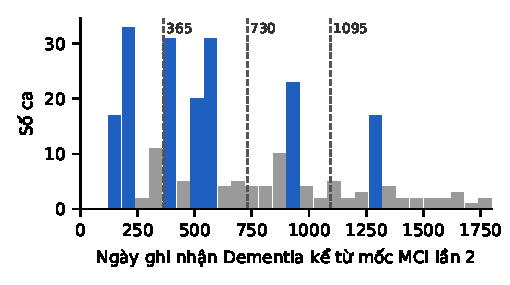
\includegraphics[width=\columnwidth]{fig1_heaping.pdf}
\caption{Ngày ghi nhận Dementia sau mốc MCI lần 2 (train). Các cụm trùng lịch khám.}
\label{fig:heap}
\end{figure}

\textit{Đặc trưng} (chỉ dùng dữ liệu có ngày $\le s$):
\begin{itemize}
\item \textbf{M0:} $\tau,\tau^2$ (năm từ MCI đầu tiên), tuổi, giới, học vấn, MMSE, FAQ, ADAS-Cog13, RAVLT trì hoãn.
\item \textbf{M1:} M0 cộng $\mathrm{HV_{adj}}$, độ dày nội khứu và chỉ báo 3T.
\item \textbf{M2:} M1 cộng slope ADAS-Cog13 và slope FAQ.
\item \textbf{M3:} M2 cộng slope hồi hải mã và slope nội khứu.
\end{itemize}
Thể tích được hiệu chỉnh theo ICV: $\mathrm{HV_{adj}}=\mathrm{HV}-b(\mathrm{ICV}-\overline{\mathrm{ICV}}_{\mathrm{CN}})$. Slope là BLUP
\begin{equation}
\hat r_i=\gamma_1+\big[DX_i^\top V_i^{-1}(y_i-X_i\gamma)\big]_2,\quad V_i=X_iDX_i^\top+\sigma^2I,
\end{equation}
tính trên các lần đo trước hoặc tại mốc, trải ≥ 300 ngày. Với MRI, chỉ dùng các lần chụp cùng phiên bản FreeSurfer và cùng cường độ từ trường.

Tham số $(b,\gamma,D,\sigma^2)$ không dùng kết cục. Chúng được gộp từ thống kê OLS tính sẵn cho từng người, nên ước lượng lại trên một tập RID bất kỳ gần như không tốn thời gian. Nhờ vậy, mọi fold ước lượng tham số chỉ từ RID không thuộc phần đánh giá, ở cả vòng trong lẫn vòng ngoài.

\textit{Tại sao tốc độ hai điểm thất bại.} Sai số của tốc độ năm hóa từ hai lần chụp có phương sai
\[
\operatorname{Var}(\hat r-r)=2\sigma^2\,\big(365{,}25/\Delta d\big)^2 .
\]
Với $\sigma\approx125$ mm³ và $\Delta d=206$ ngày (trung vị trong train), độ lệch chuẩn sai số khoảng 310 mm³/năm. Con số này lớn gấp gần 3 lần mức teo trung bình của quần thể MCI (109 mm³/năm).

\section{Mô hình và đánh giá}
Mô hình là tỷ lệ nguy cơ với nguy cơ nền hằng từng khúc: 6 khúc 182,5 ngày đến 1.095 ngày, 2 khúc 365 ngày đến 1.825 ngày và một khúc mở. Hàm log-likelihood kiểm duyệt khoảng có phạt là
\begin{equation}
\begin{aligned}
\ell={}&\textstyle\sum_k w_k\log\big[S(L_k\mid z_k)-S(R_k\mid z_k)\big]\\
&-\tfrac{\lambda}{2}\lVert\beta\rVert^2-\tfrac{\kappa}{2}\textstyle\sum_j(a_j-a_{j-1})^2,
\end{aligned}
\end{equation}
với $w_k=1/n_i$ để mỗi người có tổng trọng số bằng 1. $\lambda\in\{0{,}1;1;10\}$ được chọn bằng CV lồng 3 fold. Kiểm duyệt được mô hình hóa bằng Cox ridge~\cite{cox} có trọng số theo người.

\textit{Trạng thái tại $h$:}
\begin{itemize}
\item ca chắc chắn: $R\le h$;
\item chắc chắn chưa biến cố: $L\ge h$;
\item khoảng vắt qua ngày đích: $L<h<R$, rút $T$ từ M0;
\item ngừng theo dõi sớm: trọng số 0, hiệu chỉnh bằng IPCW.
\end{itemize}
Hình~\ref{fig:status} báo số người trong bốn nhóm.

Các chỉ số gồm td-AUC, Brier và IPA~\cite{ipa}, net benefit~\cite{dca} ($\mathrm{NB_{core}}$ là trung bình NB ở các ngưỡng 15–30\%), và hiệu chuẩn bằng Turnbull NPMLE~\cite{turnbull} trên 10 nhóm nguy cơ. Ở 730 ngày, tỷ lệ quan sát theo IPCW là 0,327, theo Turnbull là 0,287. Vì vậy hiệu chuẩn dùng Turnbull; các Δ giữa mô hình dùng chung trọng số nên vẫn so sánh công bằng.

\textit{Quy tắc kết luận} (khóa trước) cho Δ = M3 − M2:
\begin{itemize}
\item \textbf{Có giá trị gia tăng:} cận dưới ΔAUC $>0$, ΔAUC $\ge0{,}02$ và cận dưới ΔNB $>0$.
\item \textbf{Tương đương:} KTC 95\% của ΔAUC nằm trong $(-0{,}02;0{,}02)$ và cận trên ΔNB $\le0{,}01$.
\item \textbf{Bất định:} các trường hợp còn lại.
\end{itemize}
Câu tổng kết chỉ được viết ``có giá trị gia tăng'' khi cả CV và test cùng đạt nhánh đó.

\begin{figure}[t]
\centering
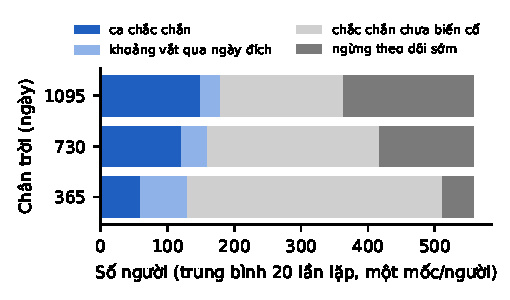
\includegraphics[width=\columnwidth]{fig4_status.pdf}
\caption{Bốn nhóm trạng thái tại từng chân trời (CV, một mốc ngẫu nhiên mỗi người).}
\label{fig:status}
\end{figure}

\section{Kết quả}
\subsection{Hiệu năng trong CV}
Tập ghép cặp gồm 558 người (1.176 mốc), trong đó 202 người có Dementia trong cửa sổ. Bảng~\ref{tab:cv} cho thấy cả bốn mô hình phân biệt tốt và hiệu chuẩn tổng thể sát (O/E Turnbull 0,93–1,03). Ở 730 ngày, NB$_{20\%}$ của các mô hình là 0,234–0,245, cao hơn chiến lược can thiệp tất cả (0,159).

\begin{table}[t]
\caption{CV lặp 5 fold × 20 lần trên train (558 người)}
\label{tab:cv}
\centering\footnotesize
\begin{tabular}{@{}llcccc@{}}
\toprule
$h$ & Mô hình & AUC & IPA & O/E & NB$_{\text{core}}$\\
\midrule
365 & M0 & 0,865 & 0,274 & 1,03 & 0,130\\
    & M3 & 0,874 & 0,294 & 1,03 & 0,138\\
730 & M0 & 0,871 & 0,356 & 0,98 & 0,225\\
    & M1 & 0,879 & 0,380 & 0,98 & 0,233\\
    & M2 & 0,880 & 0,383 & 0,98 & 0,233\\
    & M3 & 0,884 & 0,396 & 0,97 & 0,235\\
1095& M0 & 0,868 & 0,398 & 0,94 & 0,295\\
    & M3 & 0,886 & 0,448 & 0,93 & 0,305\\
\bottomrule
\end{tabular}
\end{table}

\subsection{Giá trị gia tăng, tách theo tầng}
Bảng~\ref{tab:delta} tách kết quả CV và test. Trong CV ở 730 ngày, ΔAUC của M3 − M2 là 0,004 và ΔNB là 0,002. Cả hai khoảng tin cậy nằm trong biên định trước, nên CV đạt \emph{tương đương}; ở 1.095 ngày cũng vậy. Trên test (141 người), khoảng tin cậy rộng gấp khoảng 2 lần và kết quả \emph{bất định} ở mọi chân trời. Theo quy tắc báo cáo đã khóa, kết luận chung là: \emph{chưa đủ bằng chứng về giá trị gia tăng ổn định của tốc độ MRI}.

Đóng góp lớn nhất vẫn đến từ một lần MRI (M1 − M0: +0,009 ở 730 ngày). Slope nhận thức (M2 − M1) gần như bằng 0.

\begin{table}[t]
\caption{Chênh lệch ghép cặp (KTC 95\% bootstrap cụm người)}\setlength{\tabcolsep}{3pt}
\label{tab:delta}
\centering\footnotesize
\begin{tabular}{@{}llcc@{}}
\toprule
Tầng & So sánh, $h$ & ΔAUC & ΔNB$_{\text{core}}$\\
\midrule
CV & M1 − M0, 730 & 0,009 (−0,012; 0,029) & 0,008 (−0,005; 0,021)\\
CV & M2 − M1, 730 & 0,001 (−0,005; 0,006) & 0,000 (−0,005; 0,005)\\
CV & M3 − M2, 730 & 0,004 (−0,006; 0,014) & 0,002 (−0,007; 0,009)\\
CV & M3 − M2, 1095 & 0,005 (−0,006; 0,017) & −0,001 (−0,009; 0,009)\\
Test & M3 − M2, 730 & −0,002 (−0,021; 0,018) & 0,000 (−0,010; 0,009)\\
Test & M3 − M2, 1095 & 0,003 (−0,014; 0,023) & 0,003 (−0,008; 0,018)\\
\bottomrule
\end{tabular}
\end{table}

\subsection{Kiểm toán rò rỉ và phân tích độ nhạy}
Hình~\ref{fig:forest} tóm tắt các phân tích độ nhạy. Tất cả đều chạy 20 lần lặp, có CV lồng, và đều mang tính thăm dò.
\begin{itemize}
\item \textbf{L1:} ước lượng tham số trên toàn train như ver4 cho ΔAUC 0,0047, so với 0,0042 khi ước lượng trong fold.
\item \textbf{S1 (Cox kiểm duyệt phải):} ở 365 ngày, O/E là 1,83 so với 1,02, IPA giảm từ 0,297 xuống 0,155, ΔNB là −0,052 (−0,079; −0,031).
\item \textbf{S2a:} tốc độ hai điểm cho −0,002 (−0,008; 0,002).
\item \textbf{S2b} (ADNIGO/2, 235 người): BLUP cho 0,022 (−0,001; 0,042), BSI cho 0,005. Tín hiệu báo ở ver4 (0,038 với 5 lần lặp) giảm khi chạy 20 lần lặp.
\item \textbf{S8:} khi yêu cầu MRI có trước mốc ≥ 1, 7 hoặc 30 ngày, còn lại 508, 441 hoặc 318 người, và ΔAUC đều ≈ 0,001.
\item \textbf{S9:} cửa sổ MRI 180 ngày giữ được 531 người (1.018 mốc), so với 558 người (1.176 mốc) ở cửa sổ 365 ngày. AUC của M3 ở nhóm MRI 181–365 ngày tuổi (0,896) không thấp hơn nhóm ≤ 180 ngày (0,883). Tương tác HV × tuổi MRI cho ΔAUC −0,0004.
\item \textbf{S3, S4, S5, S6, S7, S10:} Δ nằm trong khoảng 0,004–0,015, mọi khoảng tin cậy đều chứa 0.
\end{itemize}

\begin{figure}[t]
\centering
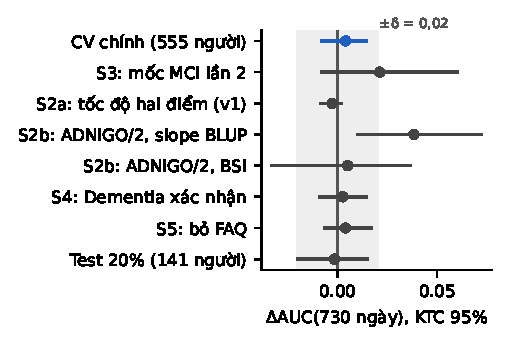
\includegraphics[width=\columnwidth]{fig2_forest.pdf}
\caption{ΔAUC ở 730 ngày (M3 − M2, hoặc biến thay thế − M2). Vùng xám là ±δ.}
\label{fig:forest}
\end{figure}

\subsection{Test và bộ mô hình theo dữ liệu hiện có}
Trên test, AUC ở 730 ngày là 0,918–0,924 và O/E Turnbull là 1,07–1,09 (Hình~\ref{fig:cal}). Slope hiệu chuẩn 1,6–1,9 dựa trên 10 nhóm, mỗi nhóm khoảng 14 người, nên kém ổn định.

Bộ mô hình dùng trong web học trên 865, 811, 604 và 558 người (M0–M3). AUC CV ở 730 ngày của bộ này lần lượt là 0,862, 0,875, 0,881 và 0,890; AUC test là 0,878, 0,884, 0,918 và 0,917.

\begin{figure}[t]
\centering
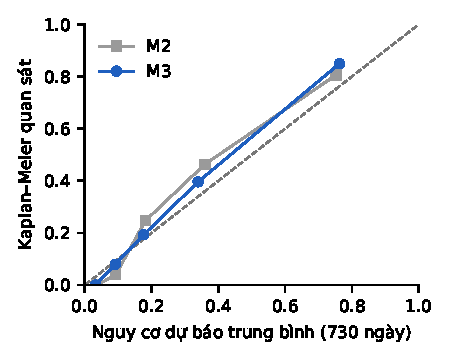
\includegraphics[width=0.85\columnwidth]{fig3_calibration.pdf}
\caption{Hiệu chuẩn trên test ở 730 ngày: 10 nhóm nguy cơ, quan sát bằng Turnbull.}
\label{fig:cal}
\end{figure}

\section{Thảo luận}
Các sửa đổi của ver5 không làm thay đổi bức tranh chung. Kiểm toán L1 xác nhận rò rỉ tiền xử lý ở ver4 có thật nhưng không đáng kể. MRI cũ đến 365 ngày không làm giảm giá trị dự báo. Độ trễ xử lý MRI không ảnh hưởng tới Δ. Điểm thay đổi thực chất là phân tích ADNIGO/2: tín hiệu dương của ver4 không đứng vững khi lặp đủ số lần.

Ở chân trời ngắn, mô hình hóa kiểm duyệt khoảng vẫn là yếu tố quyết định cho xác suất tuyệt đối (S1). Tốc độ hai điểm không dùng được vì sai số đo $\approx$125 mm³ lớn hơn mức teo hằng năm.

\textit{Giới hạn:}
\begin{itemize}
\item Test nhỏ và đã được xem qua ở các phiên bản trước~\cite{riley}.
\item λ được chọn ở cận trên của lưới (10) trong phần lớn các fold.
\item Nhãn Dementia không xác định căn nguyên; tử vong được xử lý như kiểm duyệt.
\item 97\% ảnh MRI chưa được QC thủ công.
\item ADNI không đại diện cho người Việt Nam.
\item Mô hình không áp dụng cho người đang dùng kháng thể kháng amyloid.
\end{itemize}

\section{Kết luận}
Theo giao thức đã khóa, CV cho thấy tốc độ MRI tương đương về mặt thực hành với chỉ theo dõi nhận thức, còn test bất định. Kết luận chung là chưa đủ bằng chứng về giá trị gia tăng ổn định của tốc độ MRI. Một lần MRI cùng đánh giá nhận thức – chức năng đạt AUC khoảng 0,88 ở 2 năm trong CV. Bước tiếp theo là bổ sung amyloid/CDR/APOE và p-tau217, mở rộng lưới λ, và kiểm chứng ngoài trên dữ liệu độc lập.

\begin{thebibliography}{10}\footnotesize
\bibitem{landmark} H. C. van Houwelingen, ``Dynamic prediction by landmarking in event history analysis,'' \emph{Scand. J. Stat.}, vol. 34, pp. 70--85, 2007.
\bibitem{cox} D. R. Cox, ``Regression models and life-tables,'' \emph{J. R. Stat. Soc. B}, vol. 34, no. 2, pp. 187--202, 1972.
\bibitem{turnbull} B. W. Turnbull, ``The empirical distribution function with arbitrarily grouped, censored and truncated data,'' \emph{J. R. Stat. Soc. B}, vol. 38, pp. 290--295, 1976.
\bibitem{jack2024} C. R. Jack Jr. et al., ``Revised criteria for diagnosis and staging of Alzheimer's disease: Alzheimer's Association Workgroup,'' \emph{Alzheimer's Dement.}, vol. 20, no. 8, pp. 5143--5169, 2024.
\bibitem{fda2025} U.S. FDA, ``FDA clears first blood test used in diagnosing Alzheimer's disease,'' 16 May 2025.
\bibitem{ema} European Medicines Agency, ``Leqembi (lecanemab): product information,'' 2025.
\bibitem{belder2024} C. R. S. Belder et al., ``Brain volume change following amyloid-beta immunotherapy for Alzheimer's disease: amyloid-removal-related pseudo-atrophy,'' \emph{Lancet Neurol.}, 2024.
\bibitem{tripod} G. S. Collins et al., ``TRIPOD+AI statement,'' \emph{BMJ}, vol. 385, e078378, 2024.
\bibitem{riley} R. D. Riley et al., ``Minimum sample size calculations for external validation of a clinical prediction model with a time-to-event outcome,'' \emph{Stat. Med.}, 2021.
\bibitem{dca} A. J. Vickers and E. B. Elkin, ``Decision curve analysis,'' \emph{Med. Decis. Making}, vol. 26, no. 6, pp. 565--574, 2006.
\bibitem{ipa} M. W. Kattan and T. A. Gerds, ``The index of prediction accuracy,'' \emph{Diagn. Progn. Res.}, vol. 2, 7, 2018.
\bibitem{adni} Alzheimer's Disease Neuroimaging Initiative, ``Diagnostic information,'' ADNI Documentation.
\end{thebibliography}

\end{document}
